\documentclass[a4paper]{article}
\usepackage[right=1in, left=1in, top=1in, bottom=1in]{geometry}
\usepackage{graphicx}
\begin{document}
	\title{\textbf{MACHINE LEARNING LAB}}
	\author{}
	\maketitle
	\centering{\textbf{Manish Singh CS3}}\\
	\centering{\textbf{Roll No. 17/466}}\\
	\begin{figure}[h]
		\centering
		
\includegraphics{rtu.jpeg}
	\end{figure}

	\begin{large}
		Computer Science and Engineering Department\\
	\end{large}
	\begin{Large}Rajasthan Technical University, Kota\\
	\end{Large}
\newpage
	\flushleft
	\tableofcontents
	\newpage
	\section{Problem Statement}
		Write a program to demonstrate the working of the decision tree based ID3 algorithm. Use an appropriate
    data set for building the decision tree and apply this knowledge to classify a new sample.
   \begin{math} (id3.csv) (id3_test_1.csv) (pima-indians-diabetes.csv)\end{math}
\newpage
	\section{ID3 Algorithm}
	ID3 stands for Iterative Dichotomiser 3\\
    It is a classification algorithm that follows a greedy approach by selecting a best attribute that yields maximum Information Gain(IG) or minimum Entropy(H).
    \newline
    Algorithm:\\
	1. Calculate entropy for dataset.\\
    2. For each attribute/feature\\
	\hspace{10mm}1. Calculate entropy for all its categorical values.\\
	\hspace{10mm}2. Calculate information gain for the feature.\\
	3. Find the feature with maximum information gain.\\
	4. Repeat it until we get the desired tree.
	
\newpage
	\section{Training Set}
	1. ID3 - Dataset\\
	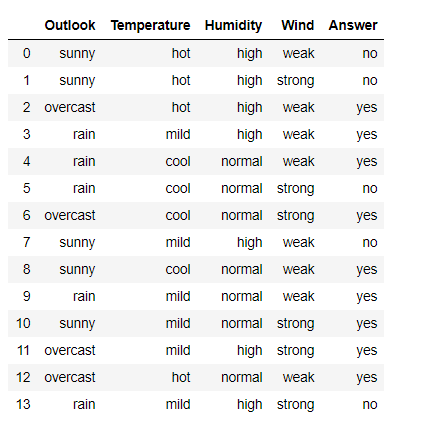
\includegraphics[scale=1.3]{id3.png}\\
	2. ID3 Test- Dataset\\
	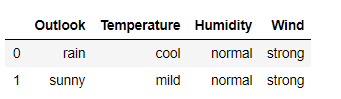
\includegraphics[scale=1.3]{id3_test_1.png}
	\newpage
	3. PIMA Indian Diabetes- Dataset
	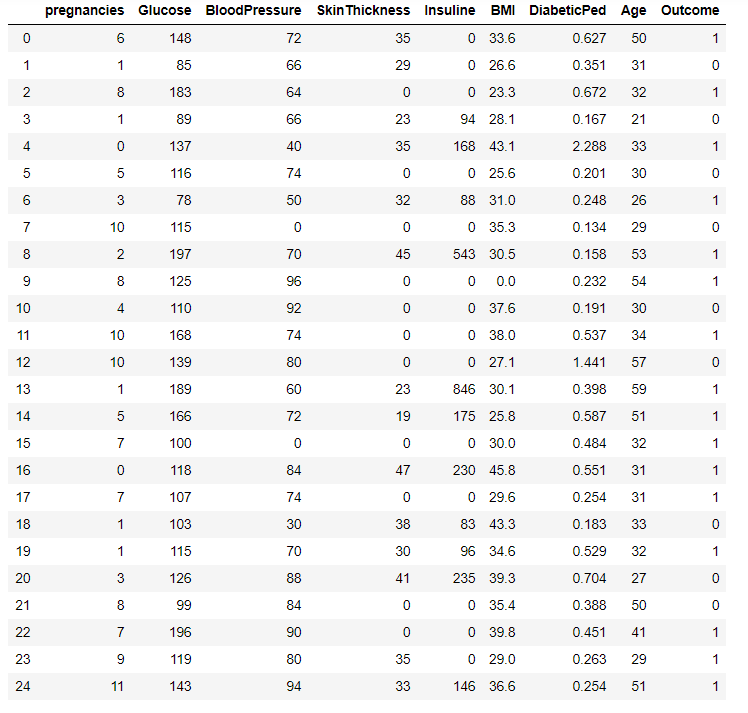
\includegraphics[scale=1.0]{pima_indian_diabetes.png}
\newpage
	\section{Program}
	\begin{verbatim}
	import numpy as np
eps = np.finfo(float).eps
from numpy import log2 as log
import pandas as pd
import pprint

df = pd.read_csv("id3.csv")
def find_entropy(df):
    Class = df.keys()[-1]   
    entropy = 0
    values = df[Class].unique()
    for value in values:
        fraction = df[Class].value_counts()[value]/len(df[Class])
        entropy += -fraction*np.log2(fraction)
    return entropy

def find_entropy_attribute(df,attribute):
    Class = df.keys()[-1]  
    target_variables = df[Class].unique()  
    variables = df[attribute].unique()    
    entropy2 = 0
    for variable in variables:
        entropy = 0
        for target_variable in target_variables:
              num = len(df[attribute][df[attribute]==variable][df[Class] ==target_variable])
              den = len(df[attribute][df[attribute]==variable])
              fraction = num/(den+eps)
              entropy += -fraction*log(fraction+eps)
        fraction2 = den/len(df)
        entropy2 += -fraction2*entropy
    return abs(entropy2)


def find_winner(df):
    Entropy_att = []
    IG = []
    for key in df.keys()[:-1]:
        Entropy_att.append(find_entropy_attribute(df,key))
        IG.append(find_entropy(df)-find_entropy_attribute(df,key))
    return df.keys()[:-1][np.argmax(IG)]
  
def get_sub_table(df, node,value):
    return df[df[node] == value].reset_index(drop=True)


def buildTree(df,tree=None): 
    Class = df.keys()[-1]   
    node = find_winner(df)
    attValue = np.unique(df[node])
    if tree is None:                    
        tree={}
        tree[node] = {}
    for value in attValue:
        sub_table = get_sub_table(df,node,value)
        clValue,counts = np.unique(sub_table[Class],return_counts=True)                        
        if len(counts)==1:
            tree[node][value] = clValue[0]                                                    
        else:        
            tree[node][value] = buildTree(sub_table) 
                   
    return tree
print("*"*20, "ID3 Algorithm to build Decision Tree","*"*20)
print("\n\nDecision Tree for the dataset ID3: \n")
t=buildTree(df)
pprint.pprint(t)
print("\n\n\n"+"*"*50)
print("\n\nDecision Tree for the dataset ID3 Test: \n")
df1 = pd.read_csv("id3_test_1.csv")
t_test = buildTree(df1)
pprint.pprint(t_test)
print("\n\n\n"+"*"*50)
print("\n\nDecision Tree for the dataset PIMA Indian Diabetes: \n")
df2 = pd.read_csv("pima_indian_diabetes.csv")
t_pima = buildTree(df2)
pprint.pprint(t_pima)
\end{verbatim}
\newpage
	\section{Output}
	\fbox{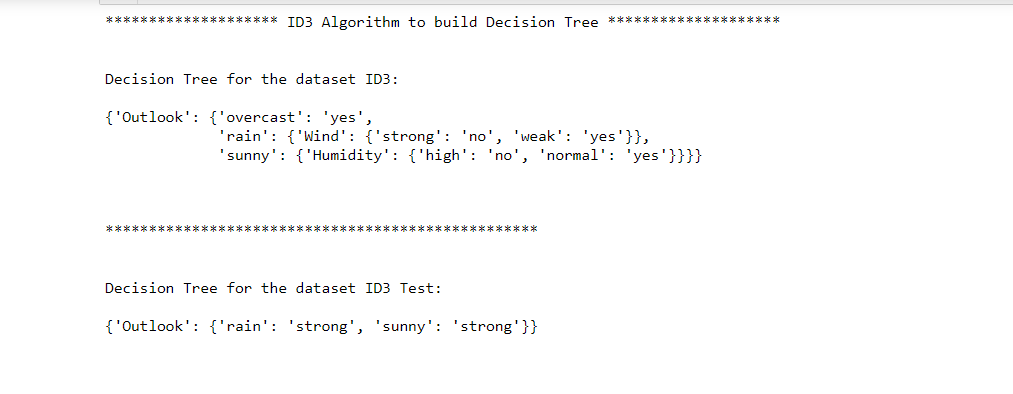
\includegraphics[width=15cm]{Screenshot (118).png}}
	\newpage
		\fbox{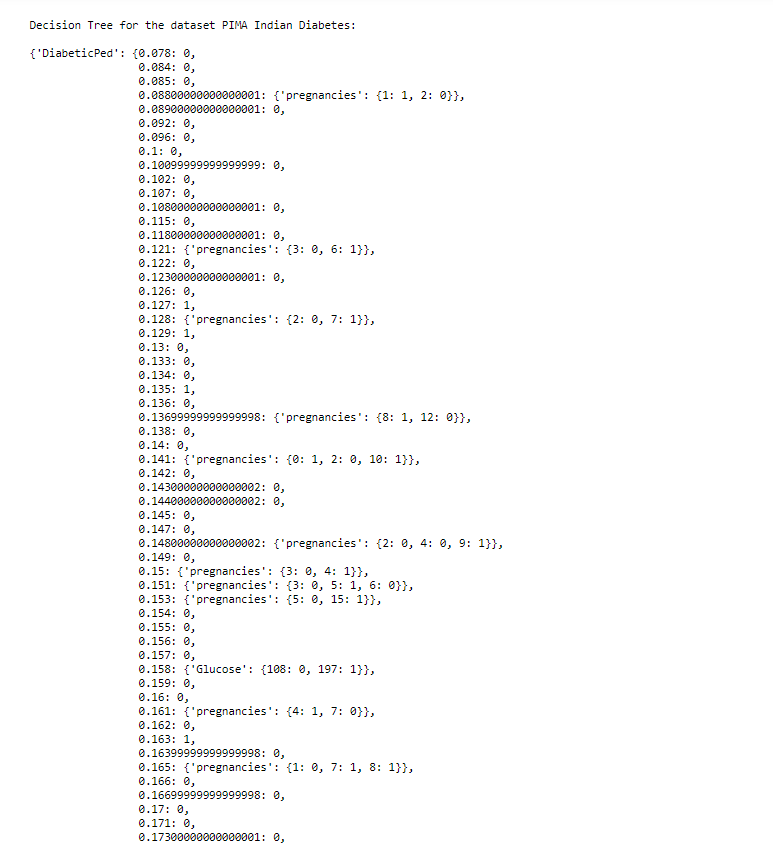
\includegraphics[width=15cm]{Screenshot (119).png}}
			\newpage
			\fbox{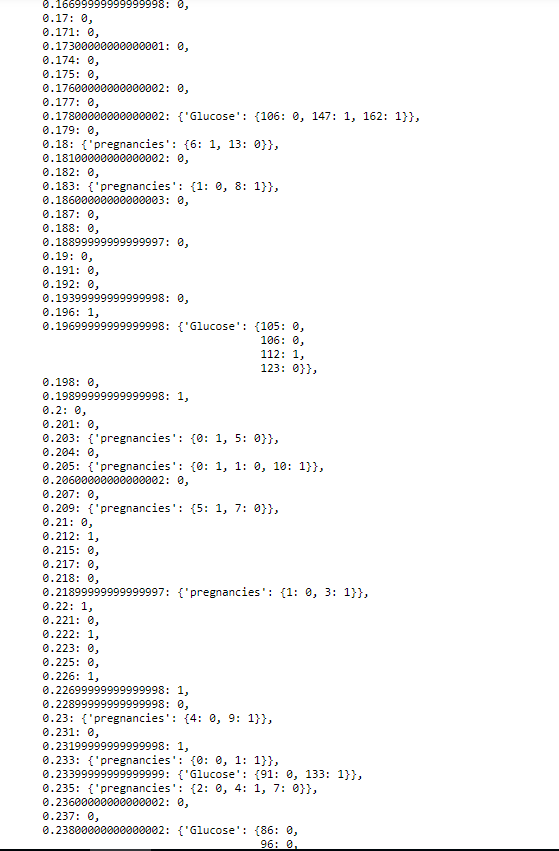
\includegraphics[width=15cm]{Screenshot (121).png}}
				\newpage
				\fbox{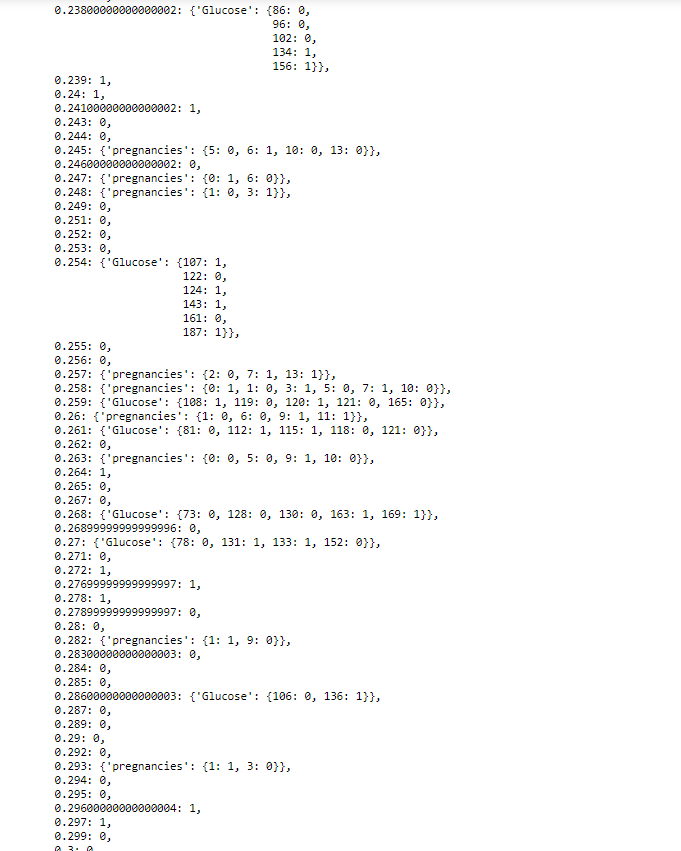
\includegraphics[width=15cm]{Screenshot (122).png}}
					\newpage
					\fbox{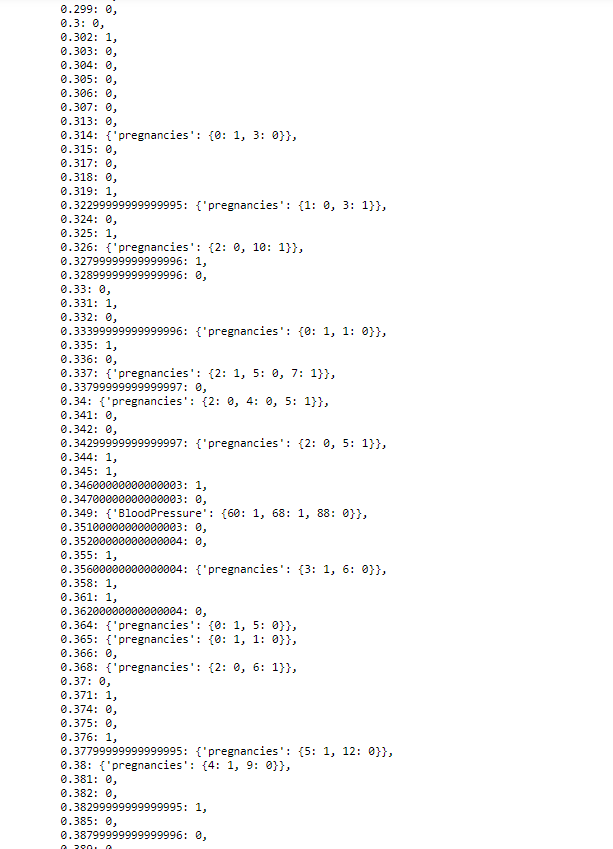
\includegraphics[width=15cm]{Screenshot (123).png}}
						\newpage
						\fbox{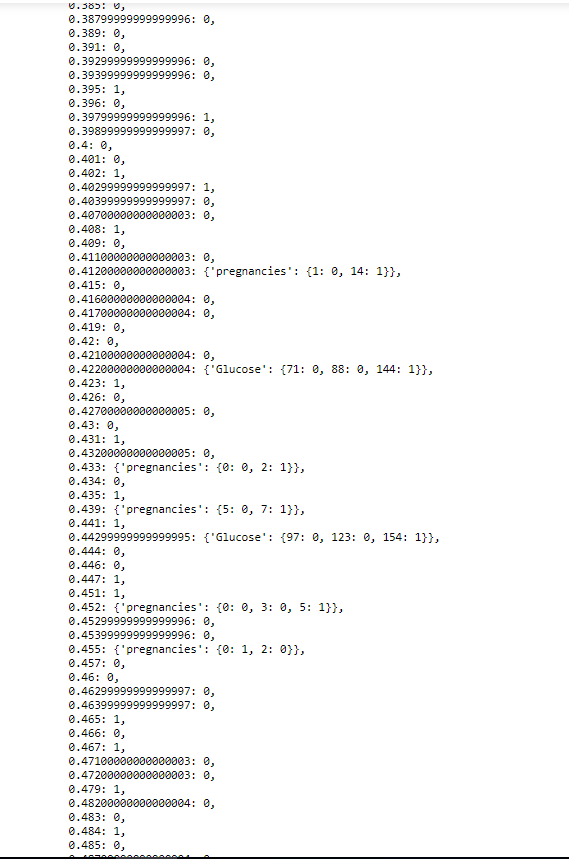
\includegraphics[width=15cm]{Screenshot (124).png}}
							\newpage
							\fbox{\includegraphics[width=15cm]{Screenshot
								(125).png}}	\newpage
								\fbox{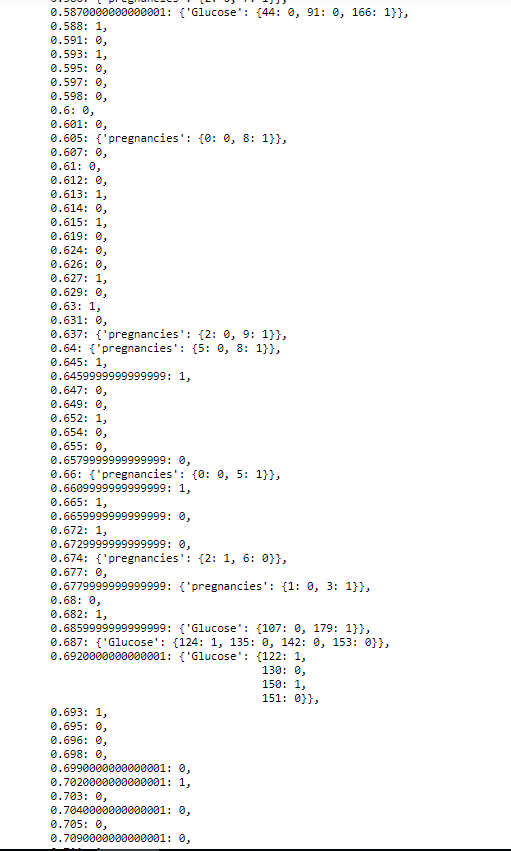
\includegraphics[width=15cm]{Screenshot (126).png}}	\newpage
									\fbox{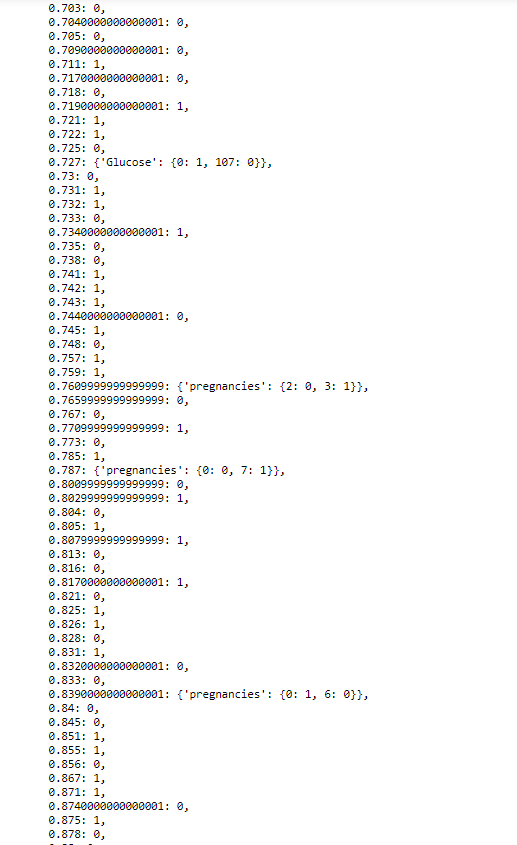
\includegraphics[width=15cm]{Screenshot (127).png}}	\newpage
							            	\fbox{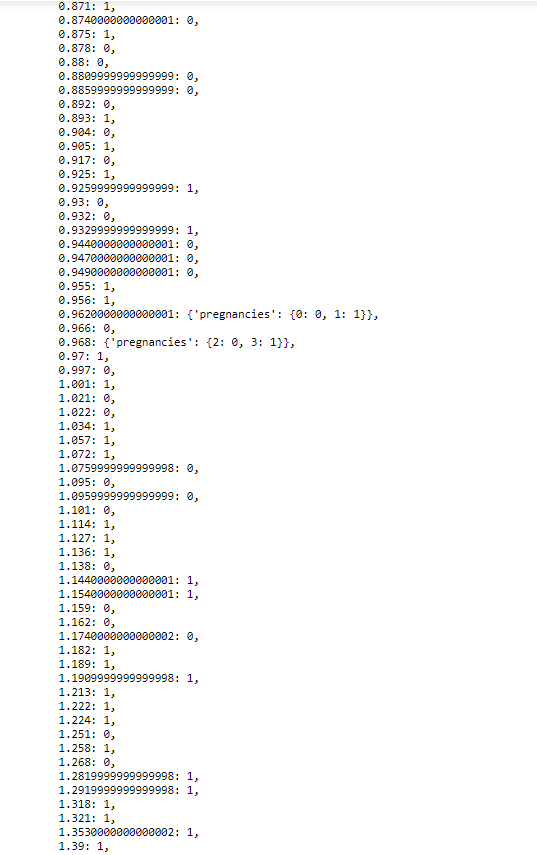
\includegraphics[width=15cm]{Screenshot (128).png}}	\newpage
							            	\fbox{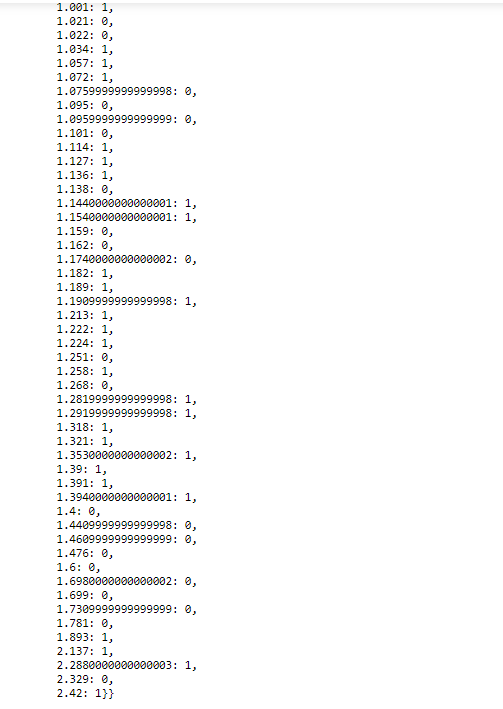
\includegraphics[width=15cm]{Screenshot (129).png}}	\newpage
	\section{Result}
	We have successfully generated the Decision Tree using ID3 algorithm for the given Data set.
\end{document}